\documentclass[11pt]{article}
\usepackage{amssymb,amsmath,amsthm,amscd,epsf,latexsym,verbatim,graphicx,amsfonts,hyperref,epstopdf,xcolor,wasysym}
\input epsf.tex
\usepackage[ruled]{algorithm2e}
\usepackage{enumerate}
\usepackage[utf8]{inputenc}
\usepackage[T1]{fontenc}
\usepackage{graphicx}
\usepackage{palatino, url, multicol}
\usepackage{subfig}
\usepackage{geometry}                % See geometry.pdf to learn the layout options. There are lots.
\usepackage{hyperref}
\geometry{letterpaper}                   % ... or a4paper or a5paper or ... 
\DeclareGraphicsRule{.tif}{png}{.png}{`convert #1 `dirname #1`/`basename #1 .tif`.png}
\usepackage{tikz,pgfplots}
\usetikzlibrary{calc,decorations.markings}
\usetikzlibrary{shapes,snakes}

% NUMBERING AND ENVIRONMENTS

\theoremstyle{plain}
\newtheorem{theorem}{Theorem}[section]
\newtheorem{conjecture}[theorem]{Conjecture}
\newtheorem{lemma}[theorem]{Lemma}
\newtheorem{prop}[theorem]{Proposition}
\newtheorem{corollary}[theorem]{Corollary}
\newtheorem{fact}[theorem]{Fact}
\newtheorem{claim}[theorem]{Claim}
\theoremstyle{definition}
\newtheorem{observation}[theorem]{Observation}
\theoremstyle{definition}
\newtheorem{defn}[theorem]{Definition}
\theoremstyle{definition}
\newtheorem{remark}[theorem]{Remark}
\theoremstyle{definition}
\newtheorem{example}[theorem]{Example}
\theoremstyle{definition}
\newtheorem{definition}[theorem]{Definition}
\theoremstyle{definition}
\newtheorem{definitions}[theorem]{Definitions}
\theoremstyle{definition}
\newtheorem{question}[theorem]{Question}
\theoremstyle{definition}
\newtheorem{outline}[theorem]{Outline of Proof}
\title{Persistent (co)homology weighted by density estimate}

\begin{document}
\maketitle

\section{Persistent Homology}

Let $X$ be a simplicial complex, $f$ a function on the faces of $X$, such that $f(\partial \sigma)\leq f(\sigma)$ for any face $\sigma$. Let $\mathcal{k}$ be a field (usually chosen to be $\mathbb{Z}/2$). Let $X(t)$ be the subcomplex consisting of faces of a value less than $t$. Then, the $i$-th persistent homology of $X$ is a sequence of vector spaces $V_t=H_k(X(t); \mathcal{k})$ and maps from $V_{t'}$ to $V_t$ for any $t'\leq t$ induced by inclusion $X(t')\subset X(t)$. The persistent homology of any finite complex can be written as a direct sum of the ``intervals'' $E_I$, which are defined as:
\[E_I(t)=\begin{cases} k & \text{ when } t\in I\\ 0 &\text{ when }t\not\in I\end{cases}\]
\[rank(E_I(t')\rightarrow E_I(t))=\begin{cases} 1 & \text{ when }t'\leq t, t', t\in I\\ 0 & \text{ otherwise }\end{cases}\]
Here $I$ is a (finite or infinite, open or closed) interval in $\mathbb{R}$. The persistent diagram of $(X, f)$ is defined as the multiset of points in $(\mathbb{R}\cup\{\pm\infty\})^2$ whose coordinates are the start and end points of the intervals.\\

A key property of the persistent homology is that it is stable \cite{CdSO}. In particular, the bottleneck distance between the diagram of $(X, f)$ and $(X, f')$ is bounded, up to a universal multiplicative constant independent from $X$, by $|f-f'|_\infty$.\\

\section{Motivation for weighting}

In many applications, there may be a need to only consider part of the complex as opposed to the whole one: for example, part of the complex may consist of points of low density, or one may want to consider localized homology and disregard the points far from a given point. \cite{B} and \cite{C} provides two different approaches to incorporate density data into persistent homology and use them to obtain robust statistics that characterizes the homology of the parts of high density. \\

However, in some situations one may want to characterizes the persistent homology of the interesting part and not just homology, which would require some kind of weighting when calculating persistent homology. In \cite{Be} a weighting is provided, but the weighting is by some ideal in a PID and not real numbers and the intuition is similar to sheaf homology and the $L^2$ theory. Here we propose another weighted version of persistent homology based on multidimensional persistent \cite{CZ, CSZ} and the ideas in \cite{B} which is conceptually simple and easy to compute and analyze.

\section{Definition}

In this paper all the limit and integral of measures are in the weak sense. Also, by $\chi(\cdot)$ we mean characteristic function for $\cdot$, $\delta_\cdot$ means Dirac mass at $\cdot$.\\

Let $X$ be a simplicial complex, $f$ and $\rho$ be two functions on the faces of $X$, so that $f(\partial\sigma)\leq f(\sigma)$, $\rho(\partial\sigma)\leq\rho(\sigma)$. Here $\rho$ is the importance weighting, with a smaller value meaning more important. Let $\rho_0$ be a value in the range of $\rho$, $\epsilon, \epsilon_0>0$. Let $X(a, b)$ be the subcomplex consisting of faces with a $f$ value no larger than $a$ and $\rho$ value no larger than $b$. \\

We define the $n$-th weighted persistent homology of $X, f, \rho$ as
\begin{equation}
V_t=\bigoplus V_t(s)=\bigoplus_{s\in [\epsilon_0,1]} im(H_n(X(t, \rho_0-s\epsilon))\rightarrow H_n(X(t, \rho_0+s\epsilon)))\}
\end{equation}

The maps between $V_t$ are defined as in persistent homology, and the ``dimension'' is defined as 
\begin{equation}
\dim(\bigoplus_s V(s))=\int_{s\in [\epsilon_0,1]}\dim V(s) ds
\end{equation}

By dualize the whole construction one can also obtain weighted persistent cohomology.\\

From this, one can define persistent diagram, persistent landscape, persistent image etc. just as in standard persistent homology. More concretely, the weighted persistent diagram for homology is a measure on $(\mathbb{R}\cup\{\pm\infty\})^2$ defined as 
\begin{equation}
\mathcal{D}=\int_{\epsilon_0}^1 \mathcal{D}_s ds
\end{equation}
where $\mathcal{D}_s=\sum_{k=1,2,\dots n_s}\delta_{(a^s_k, b^s_k)}$, and $V_\cdot(s)$ is decomposed as a direct sum of $n_s$ intervals starting at $a^s_k$ and ending at $b^s_k$. The weighted rank function and weighted persistent image are obtained by integrating the persistent landscape and image of $V_\cdot(s)$ over $s$, and weighted persistent landscape is defined using the weighted rank function.

\section{Properties}

We will now show that the weighted persistent diagram is stable with respect to the functions $f$ and $\rho$. \\

For any $a\in \mathbb{R}$, we define $f_{a,c}$ as
\begin{equation}
f_{a,c}(\sigma)=\begin{cases} f(\sigma) &\text{ when }\rho(\sigma)\leq \rho_0-c\epsilon\text{ or }f(\sigma)>a, \rho(\sigma)\leq\rho_0+c\epsilon\\ a &\text{ when }\rho_0-c\epsilon<\rho(\sigma)\leq\rho_0+c\epsilon, f(\sigma)\leq a\\ \infty &\text{ when otherwise}\end{cases}
\end{equation}

Firstly, we will give an alternative definition of weighted persistent diagram:

\begin{prop}The weighted persistent diagram can be written as
\begin{equation}
\mathcal{D}=\int\int_{\epsilon_0}^1\sum_{k=1,\dots n_{s,t}}{1\over\epsilon'}\chi(t-\epsilon'<a_k^{s,t}<t, b_k^{s,t}\geq t)\delta_{(a_k^{s,t}, b_k^{s,t})}dsdt
\end{equation}
Where the multiset $\{(a_k^{s,t}, b_k^{s,t})\}$ is the persistent diagram of $X, f_{t,s}$.
\end{prop}

\begin{proof}

By Fubini's theorem,
  \[\mathcal{D}=\int_{\epsilon_0}^1\sum_k\delta_{(a_k^{s}, b_k^{s})}ds=\int_{\epsilon_0}^1\lim_{\epsilon'\rightarrow 0}\int\sum_k{1\over\epsilon'}\chi(t-\epsilon'<a_k^{s,t}<t, b_k^{s,t}>t)\delta_{(a_k^{s,t}, b_k^{s,t})}dt ds\]
  \[=\lim_{\epsilon'\rightarrow 0}\int\int_{\epsilon_0}^1\sum_k{1\over\epsilon'}\chi(t-\epsilon'<a_k^{s,t}<t, b_k^{s,t}>t)\delta_{(a_k^{s,t}, b_k^{s,t})}dsdt\]
  To see that the second equal sign is true, for every $(a_k^s, b_k^s)$, there is a homology class that begins at $H_n(X(a_k^s,\rho_0-s\epsilon))$ and dies at $H_n(X(b_k^s, \rho_0+s\epsilon)$. By functorial property of homology this class must correspond to an interval in the persistent homology of $X, f_{t,s}$, for any $t\in (a_k^s, b_k^s)$, hence it will appear as a term in $\int\sum_k{1\over\epsilon'}\chi(t-\epsilon'<a_k^{s,t}<t, b_k^{s,t}>t)\delta_{(a_k^{s,t}, b_k^{s,t})}dt$ when $\epsilon'<b_k^s-a_k^s$. Let $\epsilon'\rightarrow 0$ this equality follows.
\end{proof}

\begin{remark}
From the proof above one see that the limit sign can be removed if one considers only the persistent diagram restricted away from the diagonal to $\{(x,y):y>x+\epsilon'\}$:
\begin{equation}
\chi(y>x+\epsilon')\mathcal{D}=\lim_{\epsilon'\rightarrow 0}\int\int_{\epsilon_0}^1\sum_{k=1,\dots n_{s,t}}{1\over\epsilon'}\chi(t-\epsilon'<a_k^{s,t}<t, b_k^{s,t}>a_k^{s,t}+\epsilon')\delta_{(a_k^{s,t}, b_k^{s,t})}dsdt
\end{equation}
\end{remark}

\begin{prop}(Stability) Let $\psi$ be any smooth continuous function of compact support and whose support is bounded away from the diagonal, let $\mathcal{D}$ and $\mathcal{D}'$ be the weighted persistent diagrams of $(X, f, \rho)$ and $(X, f', \rho')$ respectively. Then, if $|f-f'|_\infty$ and $|\rho-\rho'|_\infty$ are both smaller than some number $m$, the difference between the integration of $\psi$ on the two diagrams is bounded up to a multiple $C$, by $|f-f'|_\infty+|\rho-\rho'|_\infty$. Here both $m$ and $C$ are uniform constants independent from $X$.
\end{prop}

\begin{proof}
  First suppose $\rho=\rho'$. Then, $|f_{t,s}-f'_{t,s}|_\infty\leq |f-f'|_\infty$, hence the conclusion of the proposition follows from the previous Remark and the stability result in \cite{CdSO}.\\

  Now we suppose $f=f'$. Because $\psi$ can be approximated by sum of simple functions supported on rectangles, one only need to prove it for $\psi=\chi_{(0, a)\times (b, \infty)}$ ($\chi$ being the characteristic function) for $a<b$. By definition of weighted pesistence diagram, we have:
  \begin{equation}
\int\psi \mathcal{D}(f,\rho)=\int_{\epsilon_0}^1\sum_{a_i^s<a, b_i^s>b}1 ds
\end{equation}
Note that the summation goes through all the homology classes in $H_k(X(a, \rho_0-\epsilon_0\epsilon))$ that survived into $H_k(X(b, \rho_0+\epsilon_0\epsilon))$. For each such homology class, if it survives to both $H(X(a, \rho_0-h\epsilon))$ and $H(X(b, \rho_0+h'\epsilon))$, it will contribute to a value of $\min(h, 1)+\min(h', 1)-2\epsilon_0$ to the integral. Hence, the integral is the same as the integral of PL function
\[\psi'=(\min(1, -x)+\min(1,y))\chi_{x<-\epsilon_0, y>\epsilon_0}\]
On the persistent diagram $(X, \rho_{a,b})$, where $\rho_{a,b}$ is defined as: 
\begin{equation}
\rho_{a,b}(\sigma)=\begin{cases}(\rho(\sigma)-\rho_0)/\epsilon &\text{ when }\sigma\in X(a, \rho_0)\text{ or }X(b,\infty)\\ \infty &\text{ when }\sigma\not\in X(b,\infty)\\ 0 &\text{ when otherwise }\end{cases}
\end{equation}
Now the conclusion follows from the fact that $|\rho_{a,b}-\rho'_{a,b}|_\infty\leq {1\over \epsilon}|\rho-\rho'|_\infty$. 
\end{proof}

\subsection{Relation with kernel density estimate, kernel distance and distance to a measure}

As in \cite{C}, the function $\rho$ can be chosen as kernel density estimate, kernel distance or distance to a measure (dtm). For kernel density estimate it is a classical result by Parzen that it will converge uniformly with probability 1. The a.s. uniform convergence for kernel distance or dtm are shown in \cite{PWZ} and \cite{C} respectively.  

\section{Algorithm}

Based on Remark 4.2, we use the following algorithm to calculate the weighted persistent diagram:


\begin{algorithm}[H]
\SetAlgoLined
Let multiset $S=\emptyset$\;
\For{$c\in \{k\epsilon(1-\epsilon_0)/N\}$}{
Find the persistent barcode of $X(\infty, \rho_0-c)$ using the algorithm in \cite{CK}. Keep those of length no less than $\epsilon'$. Let $a_k$ be their start points\;
Find $N'$ non overlapping intervals $I_i=[t'_i, t_i]$ of length less than $\epsilon'$ that covers all the $a_k$\;
\For{$t$ in $\{t_i\}$}{
Let $f_{t, c}$ be defined as in (4)\;
Find the persistent barcode of $(X, f_{t,c})$ using the algorithm in \cite{CK}\;
For each barcode that has a left end point in $I_i$ and have a length no less than $\epsilon'$, let $a$, $b$ be its start and end points respectively, put $(a,b)$ into $S$.}}
Return ${1\over N'}\sum_{(a,b)\in S}\delta_{(a,b)}$.
\caption{}
\end{algorithm}


\section{Experiments and Applications}

\subsection{$\Theta$-graph}

Let $X$ be a $1200\times 1200$ cubical complex as a discretization of $[-2,2]\times[-2,2]$, with density function $\rho=\max(e^{-20(x^2+y^2-1)^2}, e^{-20y^4})$ and $f=y$. Let $\rho_0=0.6$, $\epsilon=0.3$, $\epsilon_0=0.4$ then by computation, the weighted persistence diagram has 3 components between $(-1.03,\infty)-(-1.06,\infty)$, $(-0.26,\infty)-(-0.35,\infty)$ and $(0.94,\infty)-(0.97,\infty)$, with total weight $0.6$ at each.\\

Now do random perturbation of $f$ and $\rho$ by adding a uniform error term between $(-0.05,0.05)$. The three components are moved to $(-1.08,\infty)-(-1.11,\infty)$, $(-0.2,2)-(-0.3,\infty)$ and $(0.96,2)-(1,\infty)$ with total weights $0.6$, $0.7$ and $0.6$, which is indeed $W_\infty$ close to the result without perturbation.\\

\subsection{Weighting with kernel density estimate}

Consider the $\phi$-shaped graph consisting of the unit circle and the interval from $(-1, -1)$ to $(1,1)$, pick 800 points uniformly on the circle and 800 points uniformly on the interval, add normal error with variance 0.01 to both coordinates of these 1600 points. Use kernel function 
\[K(p, q)=\max(e^{-20\|p-q\|^2}-e^{-1},0)\]
Consider the $1000\times 1000$ grid complex covering $[-2,2]\times[-2,2]$. Let $\mu$ be the kernel density estimate, $\rho(\cdot)=1-\mu(\cdot)/\mu((0,1))$. Let $\rho_0=0.6$, $\epsilon=0.1$, $\epsilon_0=0.4$. Then, the weighted persistent diagram in dimension 0 has a component near $(-1.19,\infty)$ with weight 0.6, a component near $(-1.19, -1.08)$ with weight $0.25$, and the persistent diagram in dimension 1 has a component near $(0.23,\infty)$ with weight $0.6$ and another component near $(0.79,\infty)$ with weight $0.6$. 

\subsubsection{Confidence interval via bootstrap}

As in \cite{C} we can estimate the variance and confidence interval obtained from kernel density estimate via bootstrapping. As an example, below is the dimension-1 persistent landscape for $k=0.5$ and $1.0$ of the example above and the $95\%$ confidence interval for medium obtained via bootstrapping (red and green being the upper bound, yellow and blue being the lower):

%\begin{figure}
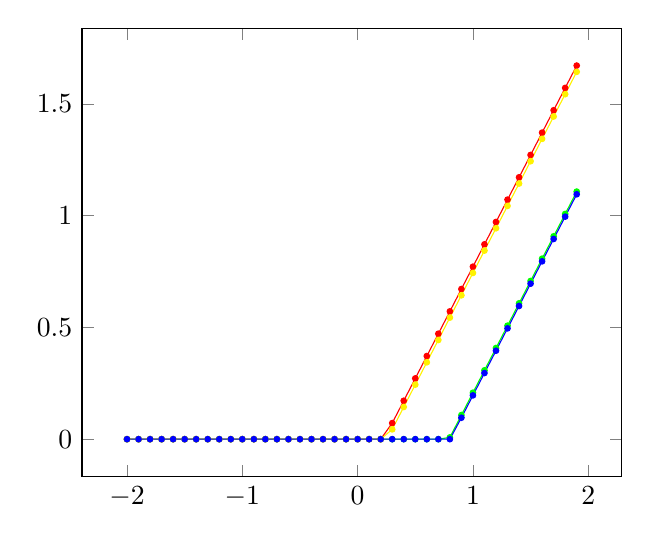
\begin{tikzpicture}
\begin{axis}[scale=1] 


\addplot[color=red,mark=*,mark size=1] coordinates {
(-2.000000, 0.000000)
(-1.900000, 0.000000)
(-1.800000, 0.000000)
(-1.700000, 0.000000)
(-1.600000, 0.000000)
(-1.500000, 0.000000)
(-1.400000, 0.000000)
(-1.300000, 0.000000)
(-1.200000, 0.000000)
(-1.100000, 0.000000)
(-1.000000, 0.000000)
(-0.900000, 0.000000)
(-0.800000, 0.000000)
(-0.700000, 0.000000)
(-0.600000, 0.000000)
(-0.500000, 0.000000)
(-0.400000, 0.000000)
(-0.300000, 0.000000)
(-0.200000, 0.000000)
(-0.100000, 0.000000)
(0.000000, 0.000000)
(0.100000, 0.000000)
(0.200000, 0.000000)
(0.300000, 0.072000)
(0.400000, 0.172000)
(0.500000, 0.272000)
(0.600000, 0.372000)
(0.700000, 0.472000)
(0.800000, 0.572000)
(0.900000, 0.672000)
(1.000000, 0.772000)
(1.100000, 0.872000)
(1.200000, 0.972000)
(1.300000, 1.072000)
(1.400000, 1.172000)
(1.500000, 1.272000)
(1.600000, 1.372000)
(1.700000, 1.472000)
(1.800000, 1.572000)
(1.900000, 1.672000)

};
\addplot[color=green,mark=*,mark size=1] coordinates {
(-2.000000, 0.000000)
(-1.900000, 0.000000)
(-1.800000, 0.000000)
(-1.700000, 0.000000)
(-1.600000, 0.000000)
(-1.500000, 0.000000)
(-1.400000, 0.000000)
(-1.300000, 0.000000)
(-1.200000, 0.000000)
(-1.100000, 0.000000)
(-1.000000, 0.000000)
(-0.900000, 0.000000)
(-0.800000, 0.000000)
(-0.700000, 0.000000)
(-0.600000, 0.000000)
(-0.500000, 0.000000)
(-0.400000, 0.000000)
(-0.300000, 0.000000)
(-0.200000, 0.000000)
(-0.100000, 0.000000)
(0.000000, 0.000000)
(0.100000, 0.000000)
(0.200000, 0.000000)
(0.300000, 0.000000)
(0.400000, 0.000000)
(0.500000, 0.000000)
(0.600000, 0.000000)
(0.700000, 0.000000)
(0.800000, 0.008000)
(0.900000, 0.108000)
(1.000000, 0.208000)
(1.100000, 0.308000)
(1.200000, 0.408000)
(1.300000, 0.508000)
(1.400000, 0.608000)
(1.500000, 0.708000)
(1.600000, 0.808000)
(1.700000, 0.908000)
(1.800000, 1.008000)
(1.900000, 1.108000)
};
\addplot[color=yellow,mark=*,mark size=1] coordinates {
(-2.000000, 0.000000)
(-1.900000, 0.000000)
(-1.800000, 0.000000)
(-1.700000, 0.000000)
(-1.600000, 0.000000)
(-1.500000, 0.000000)
(-1.400000, 0.000000)
(-1.300000, 0.000000)
(-1.200000, 0.000000)
(-1.100000, 0.000000)
(-1.000000, 0.000000)
(-0.900000, 0.000000)
(-0.800000, 0.000000)
(-0.700000, 0.000000)
(-0.600000, 0.000000)
(-0.500000, 0.000000)
(-0.400000, 0.000000)
(-0.300000, 0.000000)
(-0.200000, 0.000000)
(-0.100000, 0.000000)
(0.000000, 0.000000)
(0.100000, 0.000000)
(0.200000, 0.000000)
(0.300000, 0.044000)
(0.400000, 0.144000)
(0.500000, 0.244000)
(0.600000, 0.344000)
(0.700000, 0.444000)
(0.800000, 0.544000)
(0.900000, 0.644000)
(1.000000, 0.744000)
(1.100000, 0.844000)
(1.200000, 0.944000)
(1.300000, 1.044000)
(1.400000, 1.144000)
(1.500000, 1.244000)
(1.600000, 1.344000)
(1.700000, 1.444000)
(1.800000, 1.544000)
(1.900000, 1.644000)
};

\addplot[color=blue,mark=*,mark size=1] coordinates {
  (-2.000000, 0.000000)
(-1.900000, 0.000000)
(-1.800000, 0.000000)
(-1.700000, 0.000000)
(-1.600000, 0.000000)
(-1.500000, 0.000000)
(-1.400000, 0.000000)
(-1.300000, 0.000000)
(-1.200000, 0.000000)
(-1.100000, 0.000000)
(-1.000000, 0.000000)
(-0.900000, 0.000000)
(-0.800000, 0.000000)
(-0.700000, 0.000000)
(-0.600000, 0.000000)
(-0.500000, 0.000000)
(-0.400000, 0.000000)
(-0.300000, 0.000000)
(-0.200000, 0.000000)
(-0.100000, 0.000000)
(0.000000, 0.000000)
(0.100000, 0.000000)
(0.200000, 0.000000)
(0.300000, 0.000000)
(0.400000, 0.000000)
(0.500000, 0.000000)
(0.600000, 0.000000)
(0.700000, 0.000000)
(0.800000, 0.000000)
(0.900000, 0.096000)
(1.000000, 0.196000)
(1.100000, 0.296000)
(1.200000, 0.396000)
(1.300000, 0.496000)
(1.400000, 0.596000)
(1.500000, 0.696000)
(1.600000, 0.796000)
(1.700000, 0.896000)
(1.800000, 0.996000)
(1.900000, 1.096000)
};

\end{axis} 
\end{tikzpicture}
%\end{figure}


\subsection{Rips complex}

Let $X$ be the Rips complex built from $256$ randomly sampled points in $\{-1/2, 1/2\}^{10}$ under $L^1$ distance with threshold $3$, $f(p)=\sum_kkp_k/10$,
\[\rho(p)=e^{-2(3/2+p_0p_1 +p_3 p_4 +p_4 p_5 +p_6 p_8 +p_4 p_7 +p_8 p_9)}\]
Using the same parameters as above, one can also see clearly that the calculated weighted
persistent diagram is stable under $L^\infty$ perturbation of $\rho$ and $f$. For example, in one experiment the persistent diagram in dimension $0$ goes from being around $(-1, 1.4)$ and $(0.1, 1.4)$ and weights $0.6$, $0.35$ to around $(-1.087, 1.4)$, $(0.09, 1.4)$ with weights $0.6$, $0.05$.

\subsection{Local homology}

We can define weighted version of relative homology for a filtration \cite{dSMVJ} analogously. As local homology is a special case of relative homology filtrated by distance to a point, we can define weighted version of the local homology.\\

As an illustration, we use weighted local homology on a well studied mathematical object, the set of roots of polynomials with coefficients $\pm 1$ inside the unit circle:

\subsection{Application to shape classification}

An application is to do similar shape classification as in \cite{H} but for greyscale figures as opposed to black-and-white ones, and here the function $\rho$ is the greyscale. As an illustration, we blurred the animal figures used in \cite{H} into greyscale by convolution with characteristic functions on discs, and decrease the resolution to at most $160\times 160$, and use the weighted persistent diagram with weight being $\rho=1-g/g_{max}$, where $g$ is the gray scale, and $\rho_0=0.6$, $\epsilon=0.1$, $\epsilon_0=0.5$, as the input for their CNN. We train with batch size 64 and 60 epochs, the average accuracy is $0.69$ which is comparable to the $0.695$ average reported in \cite{H}, but with a shorter training time partly due to the lower resolution and number of epochs.

\section{Further questions and directions}

\subsection{Parameter selection}

What would be a good way to choose the parameters $\rho_0$, $\epsilon$ and $\epsilon_0$?

\subsection{Possible Application to feature selection}

Consider the Rips complexes with a fixed threshold $\alpha$. After removing certain features, the Rips complex becomes larger. Hence, one can give a weight $0$ to the faces in the small Rips complex and $1$ to the faces of the larger Rips complex that is not contained in the smaller one, and use the weighted persistent homology to measure how much of the original topological features have been preserved by deleting given features.


\begin{thebibliography}{99}
\bibitem[B]{B} Bobrowski, Omer, Sayan Mukherjee, and Jonathan E. Taylor. ``Topological consistency via kernel estimation.'' Bernoulli 23.1 (2017): 288-328.
\bibitem[Be]{Be} Bell, Greg, et al. ``Weighted Persistent Homology.'' arXiv preprint arXiv:1709.00097 (2017).
\bibitem[C]{C} Chazal, Frédéric, et al. ``Robust Topological Inference: Distance To a Measure and Kernel Distance.'' Journal of Machine Learning Research (2017).
\bibitem[CK]{CK} Chen, Chao, and Michael Kerber. ``Persistent homology computation with a twist.'' Proceedings 27th European Workshop on Computational Geometry. Vol. 11. 2011.
\bibitem[CSZ]{CSZ} Carlsson, Gunnar, Gurjeet Singh, and Afra Zomorodian. ``Computing Multidimensional Persistence.'' Algorithms and Computation: 730.
\bibitem[CZ]{CZ}Carlsson, Gunnar, and Afra Zomorodian. ``The theory of multidimensional persistence.'' Discrete \& Computational Geometry 42.1 (2009): 71-93.
\bibitem[CdSO]{CdSO} Chazal, Frédéric, Vin de Silva, and Steve Oudot. ``Persistence stability for geometric complexes.'' Geometriae Dedicata 173.1 (2014): 193-214.
\bibitem[dSMVJ]{dSMVJ} De Silva, Vin, Dmitriy Morozov, and Mikael Vejdemo-Johansson. ``Dualities in persistent (co) homology.'' Inverse Problems 27.12 (2011): 124003.
\bibitem[H]{H} Hofer, Christoph, et al. ``Deep learning with topological signatures.'' Advances in Neural Information Processing Systems. 2017.
\bibitem[PWZ]{PWZ}Phillips, Jeff M., Bei Wang, and Yan Zheng. ``Geometric Inference on Kernel Density Estimates.'' LIPIcs-Leibniz International Proceedings in Informatics. Vol. 34. Schloss Dagstuhl-Leibniz-Zentrum fuer Informatik, 2015.
\end{thebibliography}
\end{document}
